
\documentclass{beamer}
\usetheme{Singapore}
\usecolortheme[RGB={0, 32, 91}]{structure}  % Rice blue
\setbeamertemplate{navigation symbols}{\insertframenumber}

\usepackage{framed}
\usepackage{tikz}

\definecolor{riceblue}{rgb}{0.000, 0.125, 0.357}
\definecolor{ricegray}{rgb}{0.486, 0.494, 0.498}
\definecolor{ricerichblue}{rgb}{0.039, 0.314, 0.620}

\title{Player evaluation based on game performance}
\author{\color{ricerichblue} Scott Powers}


\begin{document}


\begin{frame}[noframenumbering]
  \maketitle
  \vfill
  \hfill\includegraphics[width = 4cm]{images/rice_logo.png}
\end{frame}


\begin{frame}{Outline}
  \begin{enumerate}
    \item Player evaluation based on game performance
    \begin{itemize} 
      \item Descriptive metrics
      \item Predictive metrics
    \end{itemize}
    \item Identifying undervalued players in the minor leagues w/ data
    \begin{itemize}
      \item Targeted development plans
    \end{itemize}
    \item My Research
    \begin{itemize}
      \item Basic descriptive metrics in volleyball
      \item Advanced predictive metrics in baseball
      \item Advanced descriptive metrics in soccer
    \end{itemize}
  \end{enumerate}
\end{frame}


\begin{frame}{Outline}
  \begin{enumerate}
    \item Player evaluation based on game performance
    \begin{itemize} 
      \item Descriptive metrics
      \item Predictive metrics
    \end{itemize}
    \item {\color{gray} Identifying undervalued players in the minor leagues w/ data}
    \begin{itemize}
      \color{gray}
      \item Targeted development plans
    \end{itemize}
    \item {\color{gray} My Research}
    \begin{itemize}
      \color{gray}
      \item Basic descriptive metrics in volleyball
      \item Advanced predictive metrics in baseball
      \item Advanced descriptive metrics in soccer
    \end{itemize}
  \end{enumerate}
\end{frame}


\begin{frame}{What is player evaluation?}
  ``How good is this player?''\\
  ~\\
  \begin{columns}
    \begin{column}{0.3\textwidth}
      \centering
      \includegraphics[width = \textwidth]{images/stickman_thinking.jpg}
    \end{column}
    \begin{column}{0.7\textwidth}
      Scouting and roster construction\\
      ~\\
      ~\\
      Trades and free agency\\
      ~\\
      ~\\
      The draft
    \end{column}
  \end{columns}
  ~\\
  \begin{itemize}
    \item If we add this player, how many more games will we win?
  \end{itemize}
\end{frame}


\begin{frame}{Big Picture}
  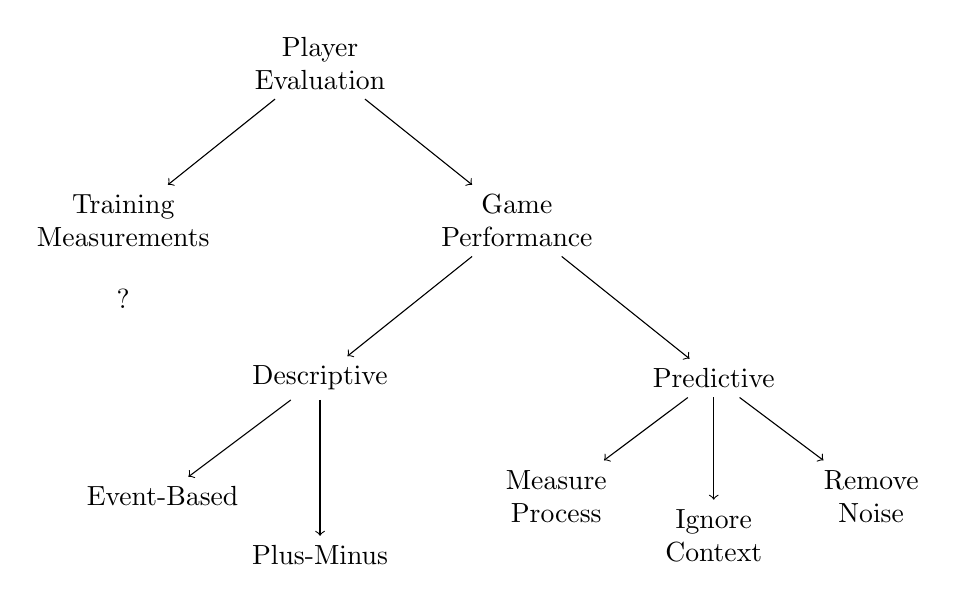
\begin{tikzpicture}
    \node[align = center] (player evaluation) at (0, 0) {Player \\ Evaluation};
    \node[align = center] (training measurements) at (-2.5, -2) {Training \\ Measurements};
    \node[align = center] (game performance) at (2.5, -2) {Game \\ Performance};
    \draw[->] (player evaluation) -- (training measurements);
    \draw[->] (player evaluation) -- (game performance);
    \pause
    \node at (-2.5, -3) {?};
    \pause
    \node (descriptive) at (0, -4) {Descriptive};
    \node (predictive) at (5, -4) {Predictive};
    \draw[->] (game performance) -- (descriptive);
    \draw[->] (game performance) -- (predictive);
    \pause
    \node (event-based) at (-2, -5.5) {Event-Based};
    \node (plus-minus) at (0, -6.25) {Plus-Minus};
    \draw[->] (descriptive) -- (event-based);
    \draw[->] (descriptive) -- (plus-minus);
    \pause
    \node[align = center] (measure process) at (3, -5.5) {Measure \\ Process};
    \node[align = center] (ignore context) at (5, -6) {Ignore \\ Context};
    \node[align = center] (remove noise) at (7, -5.5) {Remove \\ Noise};
    \draw[->] (predictive) -- (measure process);
    \draw[->] (predictive) -- (ignore context);
    \draw[->] (predictive) -- (remove noise);
  \end{tikzpicture}
\end{frame}


\begin{frame}{Big Picture}
  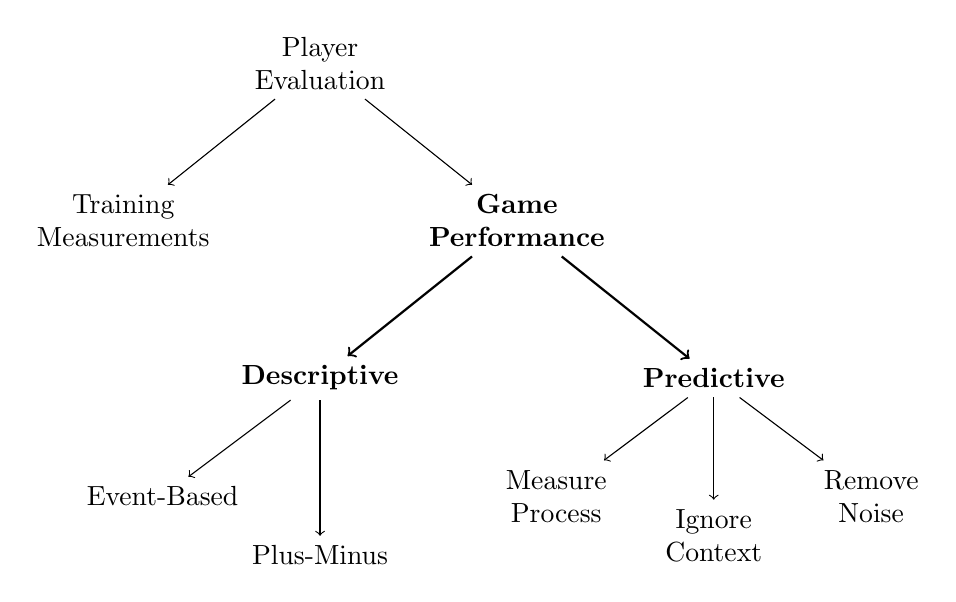
\begin{tikzpicture}
    \node[align = center] (player evaluation) at (0, 0) {Player \\ Evaluation};
    \node[align = center] (training measurements) at (-2.5, -2) {Training \\ Measurements};
    \node[align = center] (game performance) at (2.5, -2) {\bf Game \\ \bf Performance};
    \draw[->] (player evaluation) -- (training measurements);
    \draw[->] (player evaluation) -- (game performance);
    \node (descriptive) at (0, -4) {\bf Descriptive};
    \node (predictive) at (5, -4) {\bf Predictive};
    \draw[->, thick] (game performance) -- (descriptive);
    \draw[->, thick] (game performance) -- (predictive);
    \node (event-based) at (-2, -5.5) {Event-Based};
    \node (plus-minus) at (0, -6.25) {Plus-Minus};
    \draw[->] (descriptive) -- (event-based);
    \draw[->] (descriptive) -- (plus-minus);
    \node[align = center] (measure process) at (3, -5.5) {Measure \\ Process};
    \node[align = center] (ignore context) at (5, -6) {Ignore \\ Context};
    \node[align = center] (remove noise) at (7, -5.5) {Remove \\ Noise};
    \draw[->] (predictive) -- (measure process);
    \draw[->] (predictive) -- (ignore context);
    \draw[->] (predictive) -- (remove noise);
  \end{tikzpicture}
\end{frame}


\begin{frame}{Player evaluation based on game performance}
  Two guiding principles:\\
  ~
  \begin{enumerate}
    \item (Descriptive) Measure impact on team wins\\
    \begin{itemize}
      \item How do player actions cause us to win (or lose) games?
    \end{itemize}
    ~
    \item (Predictive) Separate signal from noise
    \begin{itemize}
      \item How will the player perform in the {\bf future?}
    \end{itemize}
  \end{enumerate}
  ~\\
  \pause
  Example (from {\it Moneyball}):\\
  ~\\
  \begin{columns}
    \begin{column}{0.35\textwidth}
      Batting Average = $\frac{H}{AB}$
      \begin{itemize}
        \item Less descriptive
        \item Less predictive
      \end{itemize}
    \end{column}
    \begin{column}{0.65\textwidth}
      On-Base Percentage = $\frac{H + BB + HBP}{AB + BB + HBP + SF}$
      \begin{itemize}
        \item More descriptive
        \item More predictive
      \end{itemize}
    \end{column}
  \end{columns}
\end{frame}


\begin{frame}{Big Picture}
  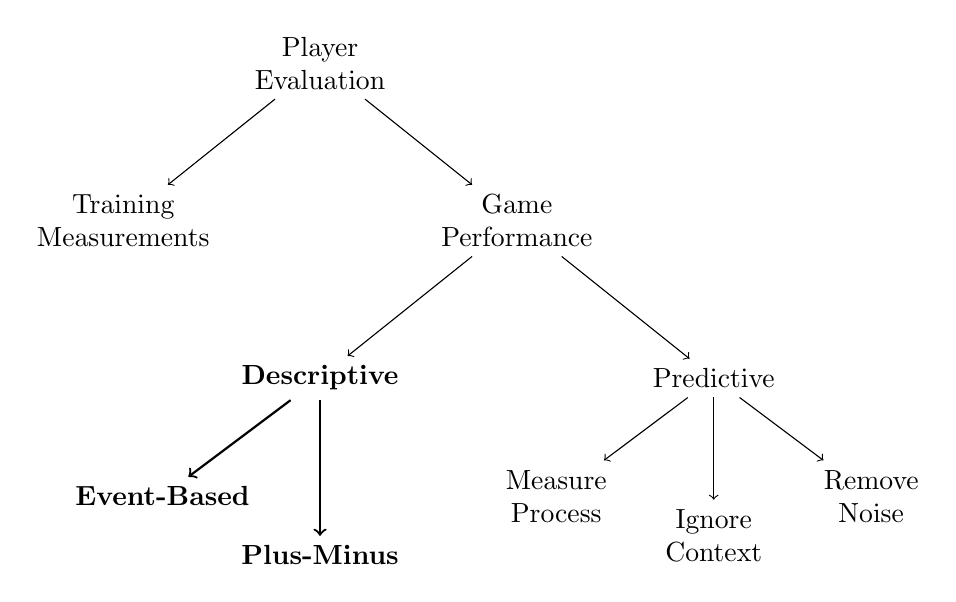
\begin{tikzpicture}
    \node[align = center] (player evaluation) at (0, 0) {Player \\ Evaluation};
    \node[align = center] (training measurements) at (-2.5, -2) {Training \\ Measurements};
    \node[align = center] (game performance) at (2.5, -2) {Game \\ Performance};
    \draw[->] (player evaluation) -- (training measurements);
    \draw[->] (player evaluation) -- (game performance);
    \node (descriptive) at (0, -4) {\bf Descriptive};
    \node (predictive) at (5, -4) {Predictive};
    \draw[->] (game performance) -- (descriptive);
    \draw[->] (game performance) -- (predictive);
    \node (event-based) at (-2, -5.5) {\bf Event-Based};
    \node (plus-minus) at (0, -6.25) {\bf Plus-Minus};
    \draw[->, thick] (descriptive) -- (event-based);
    \draw[->, thick] (descriptive) -- (plus-minus);
    \node[align = center] (measure process) at (3, -5.5) {Measure \\ Process};
    \node[align = center] (ignore context) at (5, -6) {Ignore \\ Context};
    \node[align = center] (remove noise) at (7, -5.5) {Remove \\ Noise};
    \draw[->] (predictive) -- (measure process);
    \draw[->] (predictive) -- (ignore context);
    \draw[->] (predictive) -- (remove noise);
  \end{tikzpicture}
\end{frame}


\begin{frame}{Descriptive Approach \#1: Event-Based}

  {\bf Approach:} Estimate win probability (or score expectancy) using event data. As score expectancy changes, assign credit to players responsible for those actions.\\
  ~\\
  {\bf Methods:} Markov chain (for low-dimensional game state) or machine learning (for high-dimensional game state)\\
\end{frame}


\begin{frame}{Baseball Example: Base-out run expectancy}
  \begin{center}
    \includegraphics[width = 0.5\textwidth]{images/base_out_run_expectancy.png}
    \scriptsize\color{gray} https://thebaseballscholar.com/2017/08/14/sabermetrics-101-re24/
  \end{center}
  \begin{itemize}
    \item Goal expectancy estimated via Markov chain model
    \item Bases empty, 0 out, single $= 0.831 - 0.461 = +0.370$ runs
    \item Bases loaded, 2 out, strikeout $= 0 - 0.736 = -0.736$ runs
  \end{itemize}
  ~\\
\end{frame}


\begin{frame}{Soccer Example: VAEP (Decroos et al. 2019)}
  \begin{center}
    \includegraphics[width = 0.5\textwidth]{images/vaep.png}\\
    {\scriptsize\color{gray} Decroos et al. 2019}
    \begin{itemize}
      \item Goal expectancy estimated via machine learning
    \end{itemize}
  \end{center}
  {\bf See also:} Expected Threat (Singh 2018)
\end{frame}


\begin{frame}{Descriptive Approach \#2: Plus-Minus}

  {\bf Approach:} Infer player contributions based on outcomes when they are playing vs. when they are off. Use regression to control for quality of teammates and quality of opposition.\\
  ~\\
  {\bf Methods:} Ridge regression, hierarchical Bayesian modeling, or linear mixed-effects regression
\end{frame}


\begin{frame}{Basketball Example: Regularized Adjusted Plus-Minus}
  \begin{center}
    \includegraphics[width = 0.8\textwidth]{images/rapm.png}\\
    {\scriptsize\color{gray} (Jacobs 2017)}
  \end{center}
  \begin{itemize}
     \item Works well (many substitutions and scoring events)
  \end{itemize}
\end{frame}


\begin{frame}{Soccer Example: {\bf Augmented} Adjusted Plus-Minus}
  \begin{center}
    \includegraphics[width = 0.5\textwidth]{images/aapm.png}\\
    {\scriptsize\color{gray} (Matano et al. 2023)}
    \begin{itemize}
       \item Problem: Soccer has few scoring events AND few subs
       \item Solution: Set your prior belief using additional information (e.g. video game player ratings, Matano et al. 2023)
    \end{itemize}
  \end{center}
  {\bf See also:} Box Plus-Minus (Myers 2020)
\end{frame}


\begin{frame}{Big Picture}
  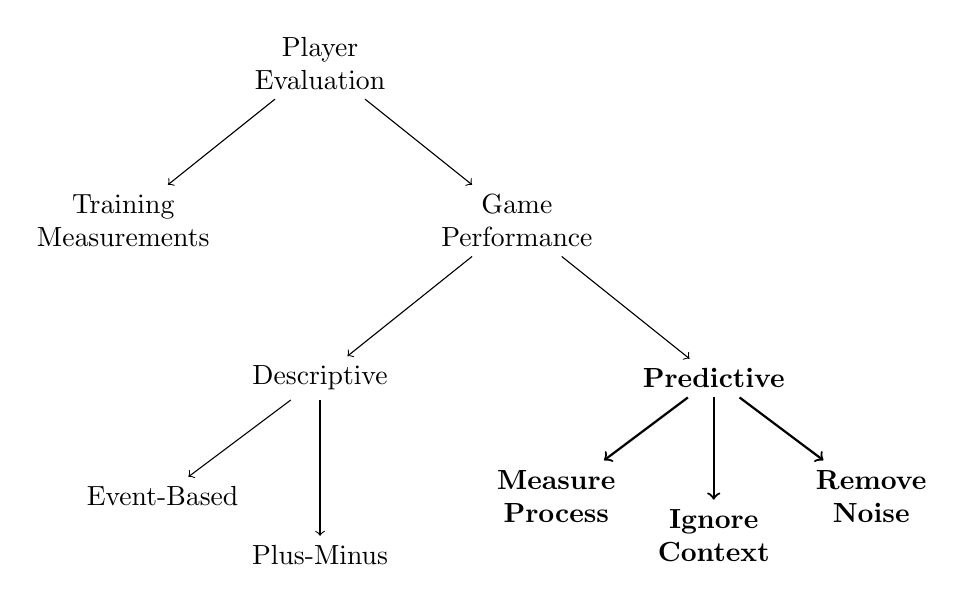
\begin{tikzpicture}
    \node[align = center] (player evaluation) at (0, 0) {Player \\ Evaluation};
    \node[align = center] (training measurements) at (-2.5, -2) {Training \\ Measurements};
    \node[align = center] (game performance) at (2.5, -2) {Game \\ Performance};
    \draw[->] (player evaluation) -- (training measurements);
    \draw[->] (player evaluation) -- (game performance);
    \node (descriptive) at (0, -4) {Descriptive};
    \node (predictive) at (5, -4) {\bf Predictive};
    \draw[->] (game performance) -- (descriptive);
    \draw[->] (game performance) -- (predictive);
    \node (event-based) at (-2, -5.5) {Event-Based};
    \node (plus-minus) at (0, -6.25) {Plus-Minus};
    \draw[->] (descriptive) -- (event-based);
    \draw[->] (descriptive) -- (plus-minus);
    \node[align = center] (measure process) at (3, -5.5) {\bf Measure \\ \bf Process};
    \node[align = center] (ignore context) at (5, -6) {\bf Ignore \\ \bf Context};
    \node[align = center] (remove noise) at (7, -5.5) {\bf Remove \\ \bf Noise};
    \draw[->, thick] (predictive) -- (measure process);
    \draw[->, thick] (predictive) -- (ignore context);
    \draw[->, thick] (predictive) -- (remove noise);
  \end{tikzpicture}
\end{frame}


\begin{frame}{Predictive Strategy \#1: Measure process, not results}

  {\bf Strategy:} Measure more granular data. Create predictions of outcomes using the more granular data. These predicted outcomes (usually) have higher signal-to-noise ratio than actual outcomes.\\
  ~\\
  {\bf Baseball Example:} Pitch outcome modeling\\
  \begin{center}
    \includegraphics[width = 0.5\textwidth]{images/pitch_tracking.jpg}
  \end{center}
  {\bf Soccer Example:} xG vs. goals
\end{frame}


\begin{frame}{Predictive Strategy \#2: Use context-neutral metrics}

  {\bf Strategy:} (Sometimes) It helps to ignore the context in which an event occurred. This happens when the value of the event is sensitive to context, but the performance of the event is not.\\
  ~\\
  {\bf Baseball Example:} Linear weights
  \begin{center}
    \includegraphics[width = 0.7\textwidth]{images/linear_weights.png}\\
    {\scriptsize \color{gray} https://library.fangraphs.com/principles/linear-weights/}
  \end{center}
\end{frame}


\begin{frame}{Predictive Strategy \#3: Extract signal from noise}

  {\bf Strategy:} Performance = Skill + Luck. Regression to the mean estimates a player's skill based on their performance. The amount of mean regression depends on the signal-to-noise ratio of the stat.
  \begin{center}
    \includegraphics[width = 0.8\textwidth]{images/rttm.png}
  \end{center}
  {\bf Soccer Example:} The average take-on success rate is $\bar p = 45\%$. If a player is successful in 30 of 46 attempts ($\hat p = 65\%$), we expect his future success rate to be $p^* = 52\%$.
\end{frame}


\begin{frame}{Big Picture}
  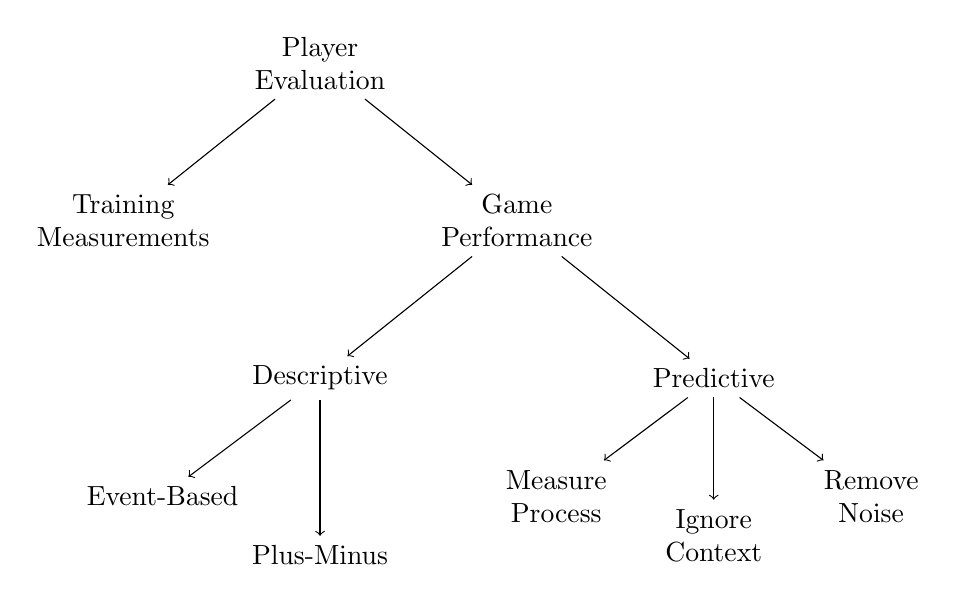
\begin{tikzpicture}
    \node[align = center] (player evaluation) at (0, 0) {Player \\ Evaluation};
    \node[align = center] (training measurements) at (-2.5, -2) {Training \\ Measurements};
    \node[align = center] (game performance) at (2.5, -2) {Game \\ Performance};
    \draw[->] (player evaluation) -- (training measurements);
    \draw[->] (player evaluation) -- (game performance);
    \node (descriptive) at (0, -4) {Descriptive};
    \node (predictive) at (5, -4) {Predictive};
    \draw[->] (game performance) -- (descriptive);
    \draw[->] (game performance) -- (predictive);
    \node (event-based) at (-2, -5.5) {Event-Based};
    \node (plus-minus) at (0, -6.25) {Plus-Minus};
    \draw[->] (descriptive) -- (event-based);
    \draw[->] (descriptive) -- (plus-minus);
    \node[align = center] (measure process) at (3, -5.5) {Measure \\ Process};
    \node[align = center] (ignore context) at (5, -6) {Ignore \\ Context};
    \node[align = center] (remove noise) at (7, -5.5) {Remove \\ Noise};
    \draw[->] (predictive) -- (measure process);
    \draw[->] (predictive) -- (ignore context);
    \draw[->] (predictive) -- (remove noise);
  \end{tikzpicture}
\end{frame}


\begin{frame}{Outline}
  \begin{enumerate}
    \item {\color{gray} Player evaluation based on game performance}
    \begin{itemize}
      \color{gray}
      \item Descriptive metrics
      \item Predictive metrics
    \end{itemize}
    \item Identifying undervalued players in the minor leagues w/ data
    \begin{itemize}
      \item Targeted development plans
    \end{itemize}
    \item {\color{gray} My Research}
    \begin{itemize}
      \color{gray}
      \item Basic descriptive metrics in volleyball
      \item Advanced predictive metrics in baseball
      \item Advanced descriptive metrics in soccer
    \end{itemize}
  \end{enumerate}
\end{frame}

\begin{frame}{Identifying undervalued players in the minor leagues}
  Framework:\\
  Player has overall skill $X$ and specific skills $X_1$, $X_2$, $X_3$.\\
  $$X = f(X_1, X_2, X_3) = X_1 + X_2 + X_3$$
  Example:
  \begin{itemize}
    \item $X$ = overall batting skill
    \item $X_1$ = plate discipline / swing decision-making
    \item $X_2$ = contact / bat-to-ball skills
    \item $X_3$ = power
  \end{itemize}
  ~\\
  If we know our coaches are particular good at developing $X_3$,\\
  what implications does that have for player acquisition?
\end{frame}

\begin{frame}{Identifying undervalued players in the minor leagues}
  Suppose our player development department can't increase $X_1/X_2$, but they can increase $X_3$ by 1 unit (run) over some time period.\\
  ~\\
  Player A: $X_1 = 1, X_2 = -1, X_3 = 1 ~~\Rightarrow X = 1$\\
  Player B: $X_1 = 1, X_2 = 1, ~~X_3 = -1 \Rightarrow X = 1$\\
  ~\\
  After player development intervention...\\
  Player A: $X_1 = 1, X_2 = -1, X_3 = 2 \Rightarrow X = 2$\\
  Player B: $X_1 = 1, X_2 = 1, ~~X_3 = 0 \Rightarrow X = 2$\\
  ~\\
  So it's a wash, unless...
  \begin{itemize}
    \item Player development can help Player B {\it more} than Player A, or
    \item $f(X_1, X_2, X_3)$ is a ``cliff'' function rather than a linear function
  \end{itemize}
\end{frame}

\begin{frame}{Outline}
  \begin{enumerate}
    \item {\color{gray} Player evaluation based on game performance}
    \begin{itemize}
      \color{gray}
      \item Descriptive metrics
      \item Predictive metrics
    \end{itemize}
    \item {\color{gray} Identifying undervalued players in the minor leagues w/ data}
    \begin{itemize}
      \color{gray}
      \item Targeted development plans
    \end{itemize}
    \item My Research
    \begin{itemize}
      \item Basic descriptive metrics in volleyball
      \item Advanced predictive metrics in baseball
      \item Advanced descriptive metrics in soccer
    \end{itemize}
  \end{enumerate}
\end{frame}


\begin{frame}{Project \#1: Basic descriptive metrics in volleyball}
  {Joint work with Luke Stancil and Naomi Consiglio}
  \begin{itemize}
    \item 4,147 matches, 600K+ points, 5M+ contacts, $\sim$6,000 players
    \item We used a Markov chain to estimate point win probability
  \end{itemize}
  ~\\
  \small\centering
  \begin{tabular}{llc|cc}
    \bf Player                      & \bf Skill                 & \bf Eval            & \bf State                   & \bf P(Sideout)\\
    \hline
    \color{red} Anna Deeber         & \color{red} Serve         &                     & \color{red} (S, SV)         & \color{orange} 57\%\\
    \color{orange} Emma Halter      & \color{orange} Reception  & \color{orange} \#   & \color{orange} (R, R\#)     & \color{orange} 63\%\\
    \color{orange} Saige K.-Torres  & \color{orange} Set        & \color{orange} \#   & \color{orange} (R, R\#S\#)  & \color{orange} 64\%\\
    \color{orange} Molly Phillips   & \color{orange} Attack     &                     & \color{orange} (R, R\#S\#A) & \color{orange} 64\%\\
    \color{red} Raquel Lazaro       & \color{red} Dig           & \color{red} +       & \color{red} (S, D+)         & \color{orange} 49\%\\
    \color{red} Elena Scott         & \color{red} Set           & \color{red} \#      & \color{red} (S, D+S\#)      & \color{orange} 47\%\\
    \color{red} Claire Chaussee     & \color{red} Attack        &                     & \color{red} (S, D+S\#A)     & \color{orange} 47\%\\
    \color{orange} Kayla Caffey     & \color{orange} Block      & \color{orange} +    & \color{orange} (R, B+)      & \color{orange} 56\%\\
    \color{red} Phekran Kong        & \color{red} Dig           & \color{red} !       & \color{red} (S, D!)         & \color{orange} 51\%\\
    \color{red} Raquel Lazaro       & \color{red} Set           & \color{red} \#      & \color{red} (S, D!S\#)      & \color{orange} 51\%\\
    \color{red} Claire Chaussee     & \color{red} Attack        &                     & \color{red} (S, D!S\#A)     & \color{orange} 51\%\\
    \hline
    \bf\color{red} Point Louisville &                           &                     &                             & \color{orange} \bf 0\%\\
  \end{tabular}
\end{frame}


\begin{frame}{Project \#1: Basic descriptive metrics in volleyball}
  {Joint work with Luke Stancil and Naomi Consiglio}
  \begin{itemize}
    \item We used a hierarchical linear mixed-effects regression to adjust each player's performance based on her quality of competition
  \end{itemize}
  \includegraphics[width = \textwidth]{images/conference_comparison.pdf}
\end{frame}


\begin{frame}{Project \#1: Basic descriptive metrics in volleyball}
  {Joint work with Luke Stancil and Naomi Consiglio}
  \centering
  \includegraphics[width = 0.6\textwidth]{images/avca_all_americans_adj.pdf}\\
  \includegraphics[width = \textwidth]{images/top_ten_players.png}
\end{frame}


\begin{frame}{Project \#2: Advanced predictive metrics in baseball}
  {Joint work with Vicente Iglesias}
  \begin{itemize}
    \item Pitch outcome modeling is very useful, but the problem is that the most important variables are the least reliable!
  \end{itemize}
  ~
  \begin{columns}
    \begin{column}{0.5\textwidth}
      \centering
      $\mbox{Variable Importance}$\\
      \includegraphics[width = \textwidth]{images/feature_importance.pdf}
    \end{column}
    \begin{column}{0.5\textwidth}
      \centering
      $\mbox{Variable Reliability}$\\
      \includegraphics[width = \textwidth]{images/feature_reliability.pdf}
    \end{column}
  \end{columns}
\end{frame}


\begin{frame}{Project \#2: Advanced predictive metrics in baseball}
  {Joint work with Vicente Iglesias}
  \begin{columns}
    \begin{column}{0.35\textwidth}
      We used a Bayesian hierarchical model to estimate the probability distribution over the 9-dimensional pitch trajectory for each pitcher in each count.\\
      ~\\
      We predicted future pitcher outcomes using this model.
    \end{column}
    \begin{column}{0.65\textwidth}
      \includegraphics[height = \textwidth]{images/656302_SL_R_plate.png}
    \end{column}
  \end{columns}
\end{frame}


\begin{frame}{Project \#2: Advanced predictive metrics in baseball}
  {Joint work with Vicente Iglesias}
  \centering
  \includegraphics[width = 0.8\textwidth]{images/cor_by_sample_size.pdf}
  \begin{itemize}
    \item Our {\bf predictive} model outperforms mean-regressed pitch outcome model for pitchers with $< 300$ pitches.
  \end{itemize}
\end{frame}
 

\begin{frame}{Project \#3: Advanced predictive metrics in soccer}
  {Joint work with Andrew Kang}
  {\bf Motivation:} Parma-led proposal for 2024 Opta Forum
  \begin{framed}
    \small\it
    Using a combination of Opta Vision events, and spatial tracking data captured for all on-field players, propose a method for categorising players, based on role-specific performance traits, to group similar stylistic players to help enhance a recruitment profiling pipeline. 
  \end{framed}
  \begin{itemize}
    \item BUT we had only 100 games of (anonymized) data
    \item We clustered players and fit cluster-specific box plus-minus
    \begin{itemize}
      \item This identifies players well-suited for specific game models
    \end{itemize}
    \item Andrew presented this work at Opta Forum!
  \end{itemize}
\end{frame}


\begin{frame}{Project \#3: Advanced predictive metrics in soccer}
  {Joint work with Andrew Kang}
  \begin{itemize}
    \item Step 1: Cluster players based on {\it style}, not performance
  \end{itemize}
  \centering
  \includegraphics[width = 0.6\textwidth]{images/opta_clusters.png}
\end{frame}


\begin{frame}{Project \#3: Advanced predictive metrics in soccer}
  {Joint work with Andrew Kang}
  \begin{itemize}
    \item Step 2: Evaluate player performance relative to their style
  \end{itemize}
  ~\\
  \includegraphics[width = \textwidth]{images/opta_bpm.png}
\end{frame}


\begin{frame}{Outline}
  \begin{enumerate}
    \item Player evaluation based on game performance
    \begin{itemize}
      \item Descriptive metrics
      \item Predictive metrics
    \end{itemize}
    \item Identifying undervalued players in the minor leagues w/ data
    \begin{itemize}
      \item Targeted development plans
    \end{itemize}
    \item My Research
    \begin{itemize}
      \item Basic descriptive metrics in volleyball
      \item Advanced predictive metrics in baseball
      \item Advanced descriptive metrics in soccer
    \end{itemize}
  \end{enumerate}
\end{frame}


\begin{frame}
  \centering
  \LARGE
  Thank You!
\end{frame}


\begin{frame}{References}
  \footnotesize
  Decroos, T., Bransen, L., Van Haaren, J., \& Davis, J. (2019). Actions speak louder than goals: Valuing player actions in soccer. In Proceedings of the 25th ACM SIGKDD international conference on knowledge discovery \& data mining (pp. 1851-1861).\\
  ~\\
  Jacobs, J. (2017). Deep Dive on Regularized Adjusted Plus-Minus I: Introductory Example. https://squared2020.com/2017/09/18/deep-dive-on-regularized-adjusted-plus-minus-i-introductory-example/\\
  ~\\
  Matano, F., Richardson, L., Pospisil, T., Politsch, C. A., \& Qin, J. (2023). Augmenting adjusted plus-minus in soccer with FIFA ratings. Journal of Quantitative Analysis in Sports, 19(1), 43-49.\\
  ~\\
  Myers, D. (2020). About Box Plus/Minus (BPM). https://www.basketball-reference.com/about/bpm2.html\\
  ~\\
  Singh, K. (2018). Introducing Expected Threat (xT). https://karun.in/blog/expected-threat.html\\
\end{frame}


\end{document}